\subsubsection{Horizontale Ausrichtung} %\subsubsection{Stelleinheit}
Um die Abwurfeinheit zum Ziel auszurichten, wird ein verstellbarer Mechanismus benötigt, der eine hohe Genauigkeit aufweist. Der Drehpunkt muss sich möglichst unter den Schwungrädern befinden, damit die 
Position des Abwurfes im Zentrum des Spielfeldes bleibt. Die Drehung wird mit einen Schrittmotor
realisiert. Ein Schrittmotor bietet sich hier an, da somit eine sehr exakte Ansteuerung gewährleistet
wird. Dadurch kann der Verstellwinkel, welcher von der Position des Zieles abhängt, genau eingestellt
werden. Der Schrittmotor wird in der Abwurfeinheit angebracht und treibt ein Ritzel an, welches in
einen Zahnkranz eingreift. Dadurch kann die Abwurfeinheit gedreht werden. Dies ist in Abbildung 
\ref{fig:GrafikDesAntriebes} ersichtlich. Damit die Bauhöhe nicht
zusätzlich vergrössert wird, ist der Zahnkranz in die Bodenplatte integriert. Die Bodenplatte mit dem
Zahnkranz reicht nicht über die ganze Abwurfeinheit, damit die Masse möglichst klein gehalten werden
kann. Der Schrittmotor ist nach dem folgenden Drehmoment von ca. $2 Nmm$ ausgelegt. Dies ist sehr klein,
da nur der Reibungskoeffizient und die Normalkraft, welche vom Gewicht der Abwurfeinheit abhängt, das
Moment erzeugen. Der Reibungskoeffizient wird durch die Lagerung klein gehalten. Die Lagerung erfolgt
im Drehzentrum durch eine Hülse und im Endbereich der Abwurfeinheit durch zwei Kugelrollen, welche mit
einem seitlichen Abstand angebracht sind. Dadurch kann ein Auflagefläche verbreitert werden, das allfälliges kippen der Abwurfeinheit verhindert. Die Ansteuerung der Schrittmotoren erfolgt über den selbst konstruierten Controller, der in der schwarzen Box, siehe Abbildung \ref{fig:GrafikDesAntriebes}, untergebracht ist.
\begin{figure}
	\centering
	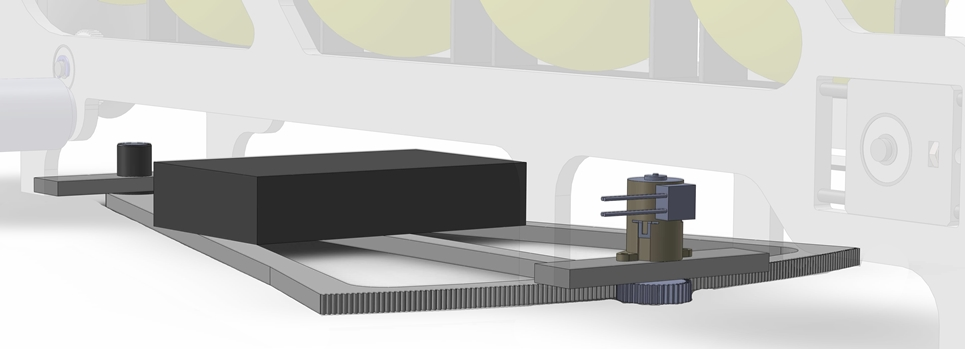
\includegraphics[width=0.9\textwidth,clip,trim=0mm 0mm 0mm 0mm]
	{Enddokumentation/Loesungskonzept/Bilder/Stelleinheit.jpg}
	\caption{Grafik des Antriebes}
	\label{fig:GrafikDesAntriebes}	
\end{figure}